\documentclass[11pt]{amsart}
\addtolength{\textheight}{3cm}
\addtolength{\textwidth}{4cm}
\addtolength{\oddsidemargin}{1cm}
\addtolength{\evensidemargin}{1cm}
\addtolength{\topmargin}{1cm}
\calclayout
\usepackage{hyperref}
\usepackage{tikz}
\usepackage{amsrefs}
\usetikzlibrary{
	hobby,
	shapes.geometric,
	calc,
	arrows,
	topaths,
	positioning
}
\usepackage{etoolbox,refcount}
\usepackage{multicol}

\newcounter{countitems}
\newcounter{nextitemizecount}
\newcommand{\setupcountitems}{%
  \stepcounter{nextitemizecount}%
  \setcounter{countitems}{0}%
  \preto\item{\stepcounter{countitems}}%
}
\makeatletter
\newcommand{\computecountitems}{%
  \edef\@currentlabel{\number\c@countitems}%
  \label{countitems@\number\numexpr\value{nextitemizecount}-1\relax}%
}
\newcommand{\nextitemizecount}{%
  \getrefnumber{countitems@\number\c@nextitemizecount}%
}
\newcommand{\previtemizecount}{%
  \getrefnumber{countitems@\number\numexpr\value{nextitemizecount}-1\relax}%
}
\makeatother    
\newenvironment{AutoMultiColItemize}{%
\ifnumcomp{\nextitemizecount}{>}{3}{\begin{multicols}{2}}{}%
\setupcountitems\begin{itemize}}%
{\end{itemize}%
\unskip\computecountitems\ifnumcomp{\previtemizecount}{>}{3}{\end{multicols}}{}}

\begin{document}
	
\title[The Bakery]{Task 1: The Bakery\\ NICD Newcastle technical interview}
\author[Mihail Hurmuzov]{Mihail Hurmuzov\\\quad\\{\normalfont\href{https://github.com/mhurmu/technical_assignment}{Github repository}}}

\maketitle

\section{Data preparation}

As the main aim of the bakery is to better predict how much goods it needs to produce each day and minimise waste, the first step we take here is to categorise all items. Every item has been coded as one of:
\begin{AutoMultiColItemize}
    \item Bread,
    \item Pastry,
    \item Packaging,
    \item Sandwich,
    \item Cake,
    \item Drink,
    \item Sweet, or
    \item Prepared meal.
\end{AutoMultiColItemize}

We assign a \emph{quantity} to each item as part of its category. An obvious illustration of this is that ``ROYAL 4P" and ``ROYAL 6P" refer to the number of pieces of the layered chocolate mousse Royal cake the customer has bought; these will be assigned $4$ and $6$ in the coding, respectively. Next, the sales data is transformed so that for each day and each category, we have a number of units in that category sold.

The idea of this approach is that a Fraisier cake and a Trois Chocolat are more likely to be interchangeable for both the bakery and for its customers than a Palet Breton and a baguette.
Moreover, a Banette might need roughly the same amount of ingredients as two Banettine, so they are given appropriate weights in the coding. As predicting each individual product is both unfeasable and potentially misleading, our method performs aggregated product sales forecasting that is more actionable without losing too much predictive power (see \cite{chan}). 

The full codebook can be found \href{https://github.com/mhurmu/technical_assignment/blob/main/Bakery%20coding.csv}{here}.

\section{Modelling}

For each product category we include as predictors:
\begin{AutoMultiColItemize}
    \item the day of the week,
    \item the month,
    \item the number of days the bakery will be closed from tomorrow,
    \item the number of days the bakery was closed until yesterday,
    \item the sales in the product category for the last two open days,
    \item the average and maximum temperature, the precipitation, the wind speed, and the snow coverage for the previous two days, the current day, and the following day.
\end{AutoMultiColItemize} 

Previous studies support the lagging of weather data, alongside the influence of future weather expectations on customer behaviour (\cite{chan}).

We fit $8$ random forest models, one for each category, on the first $80\%$ of the data and test them on the last $20\%$. On the most popular category -- bread -- the model achieves mean absolute percentage error (MAPE) of just under $13\%$ (see Figure \ref{bread} for a graph of the predictions).

\begin{figure}[h]
\[\begin{tikzpicture}
    \node (1) at (0,0) {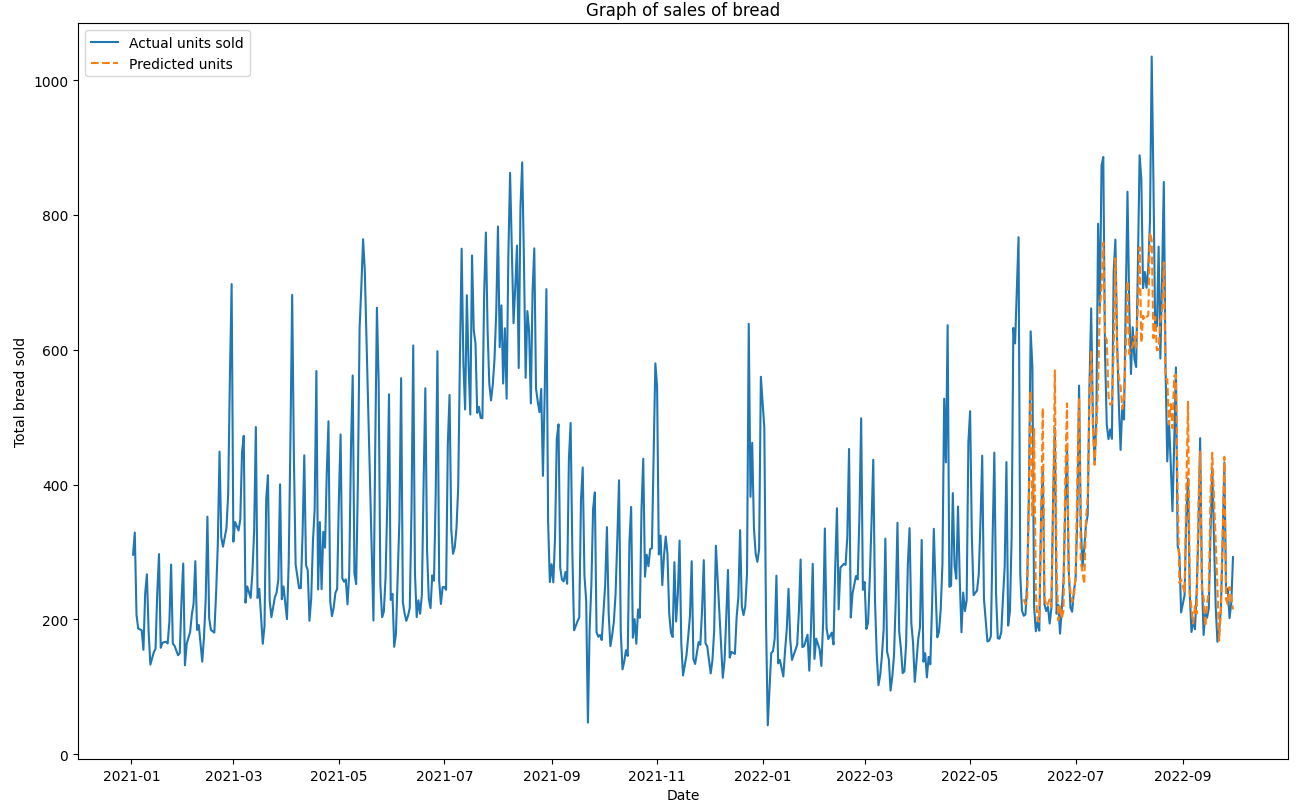
\includegraphics[scale=.45]{bread_predict.png}};
\end{tikzpicture}\]
\caption{Bread units actual vs predicted.}
\label{bread}
\end{figure}

The second most popular category, pastry, has MAPE of ${\sim}20\%$ (see top of Figure \ref{total}), while the smaller categories like cake and sweet achieve MAPE of $69\%$ and $54\%$, respectively. When the $8$ predictions are aggregated, the overall unit sales forecast has MAPE of $14.7\%$ (bottom of Figure \ref{total}).

\begin{figure}[h]
\[\begin{tikzpicture}
    \node (1) at (0,0) {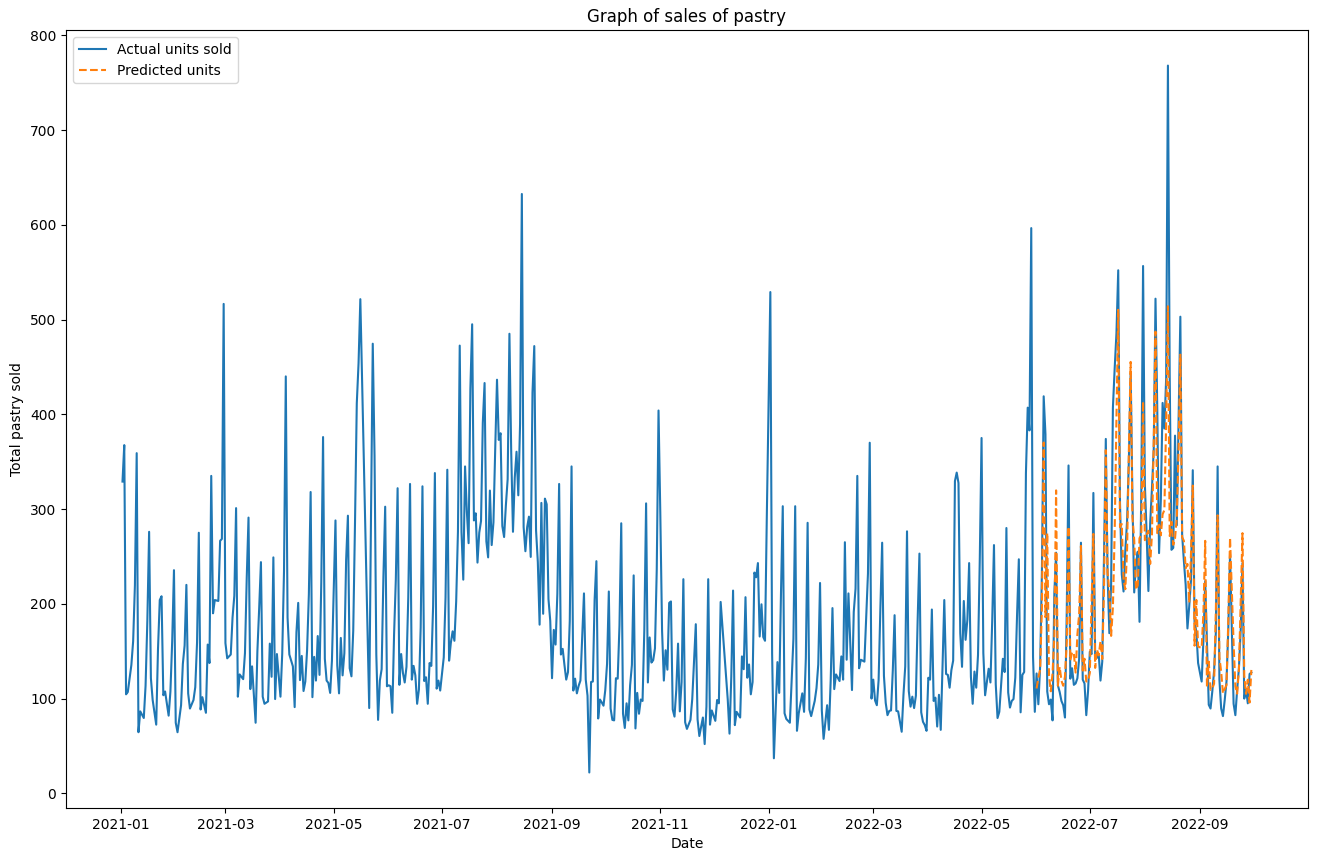
\includegraphics[scale=.45]{pastry_predict.png}};
\end{tikzpicture}\]
\[\begin{tikzpicture}
    \node (1) at (0,0) {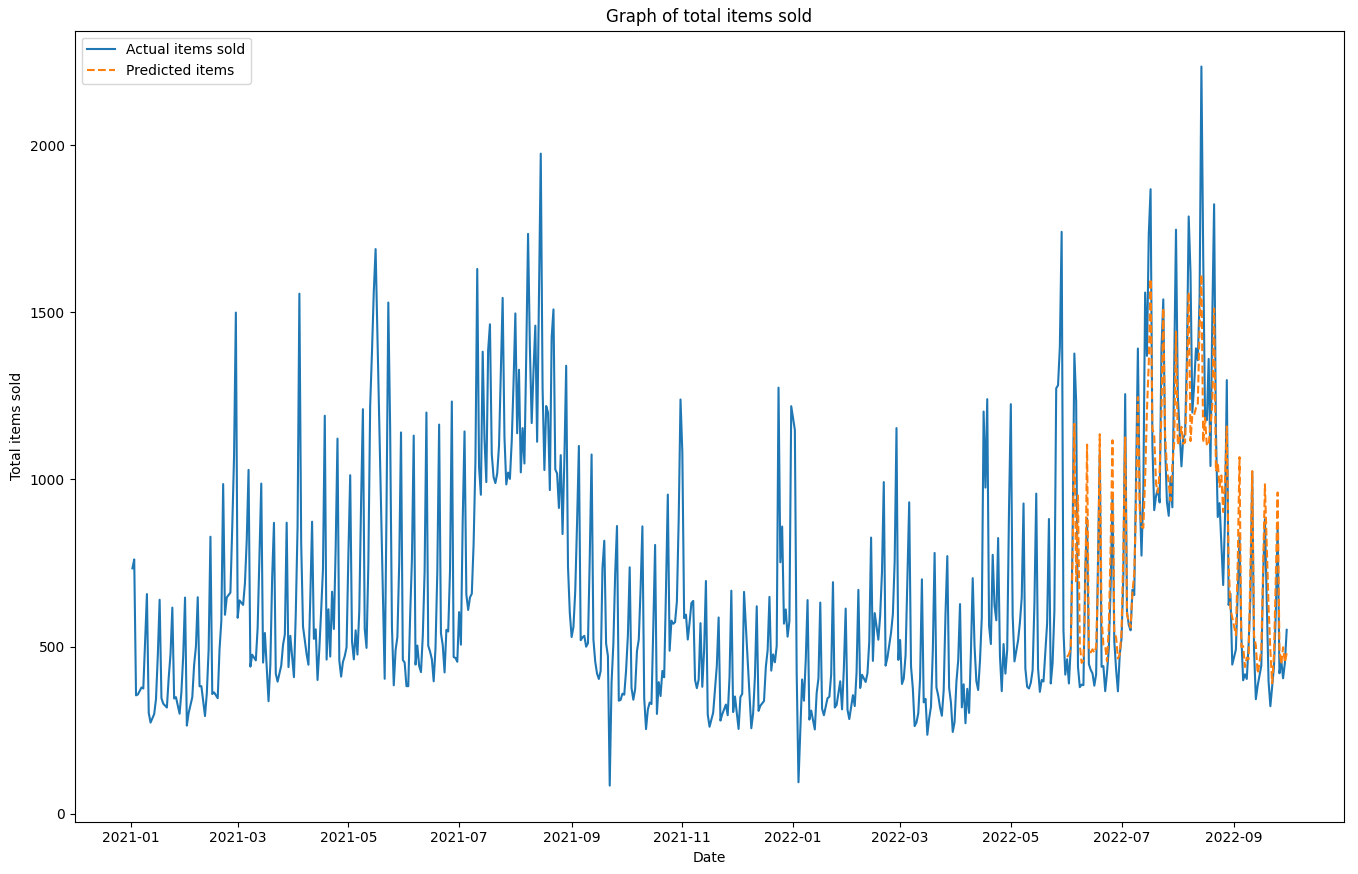
\includegraphics[scale=.45]{total_predict.png}};
\end{tikzpicture}\]
\caption{Total units actual vs predicted.}
\label{total}
\end{figure}


\section{Summary and limitations}
The codebook would ideally be developed in collaboration with the client to match their processes more closely. Additionally, information on promotional campaigns, special events, etc., could improve the model's performance, particularly during very busy periods.

While a time-series approach seems more appropriate for this problem, the intermittent nature of the sales data makes it difficult to directly account for seasonality. Even Meta's top-of-the-line \emph{prophet} module gave significantly worse results. Some of the literature also suggests that similar predictive tasks are better addressed with random forests (\cite{raizada}).

The results used in this report can be reproduced with the code supplied at the github repository \href{https://github.com/mhurmu/technical_assignment}{https://github.com/mhurmu/technical\_assignment}.


\section*{Bibliography}

\begin{biblist}

\bib{chan}{article}{
title = {A machine learning framework for predicting weather impact on retail sales},
journal = {Supply Chain Analytics},
volume = {5},
pages = {100058},
year = {2024},
issn = {2949-8635},
doi = {https://doi.org/10.1016/j.sca.2024.100058},
url = {https://www.sciencedirect.com/science/article/pii/S2949863524000013},
author = {H. Chan},
author = {M.I.M. Wahab}
}

\bib{raizada}{article}{
author = {Raizada, Stuti},
author = {Saini, Jatinderkumar},
year = {2021},
month = {01},
pages = {},
title = {Comparative Analysis of Supervised Machine Learning Techniques for Sales Forecasting},
volume = {12},
journal = {International Journal of Advanced Computer Science and Applications},
doi = {10.14569/IJACSA.2021.0121112}
}

\end{biblist}

\end{document}
